\subsubsection{10.01.2016 (Discussion)}
\textit{\textbf{Time frame:}} 16:00-20:00 

Today the cables at the elevator were held in a new way (figure \ref{Elevator3.3}). As the construction couldn't be tested by motors (the coils weren't recreated yet), it was tried by the arms. There were not noticed any problems.

\begin{figure}[H]
	\begin{minipage}[h]{1\linewidth}
		\center{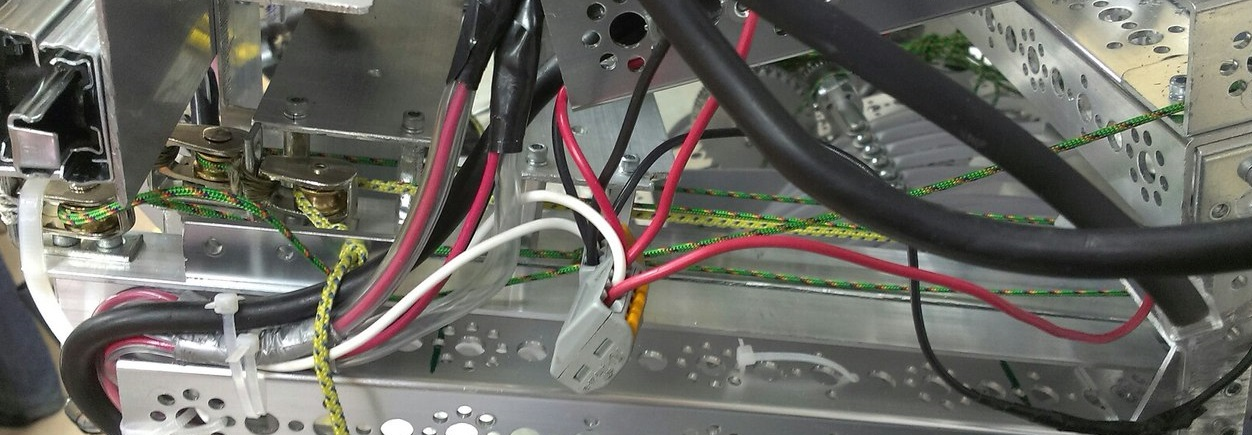
\includegraphics[scale=0.2]{3Engineering/5Team_meetings/days_of_meetings/2016.01.10/images/01}}
		\caption{Cables are held in a new way}
		\label{Elevator3.3}
	\end{minipage}
\end{figure}

The bucket was detached from the elevator to provide separate development of the bucket and the elevator.
Also results of holidays work was discussed and new tasks were set. The following table (Table ~\ref{tabular:meetingSPB10.01}) shows new tasks.

Main theme of meeting was discussing of working plans for winter holidays. As a result of it was made the following table of tasks.
\begin{table}[H]
	\caption{Results of discussion of work on holidays}
	\label{tabular:meetingSPB10.01}
	\begin{center}
		\begin{tabular}{|p{0.12\linewidth}|p{0.3\linewidth}|p{0.38\linewidth}|c|}
		  \hline 
		  \textbf{Module} & \textbf{Problem} & \textbf{Solution} & \textbf{Responsible} \\
		  \hline 
		  Lift	& Motors are not powerful enough & Make simultaneous separation &	Nikita \\
		  \hline
		  Bucket & Bucket skews while shifting & Create part in CREO, taking maximum slats bending angle into account & Sasha \\
		   & Shape and size are not optimal & Change the bucket (after drawing new shape) &	Sasha \\
		  \hline
		  Grab	& Module is not done & Finish module without small cogwheel	& Andrey \\
		  & or think of and draw construction with small cogwheel	& Andrey \\
		  \hline
		  Autonomous alpinists mechanism & Radial play of the servo mount & Fix the mount better & Andrey \\
		  \hline
		  Autonomous period & No button push & Think about it & Everyone\\
		  & No autonomous period programm	& Create and test & Andrey\\	
		  \hline
		  Crossbar engagemant & Not done, but needed & Draw and make Nikita's idea & Nikita \\
		  \hline
		\end{tabular}
	\end{center}
\end{table}
